\chapter{Methods}


\textit{\textendash\ ``Open the gates now. Private, lower your weapon''. \\ 
\textendash\ ``Not till we feed these people. Court martial me, sir. Do whatever you want with me but not till those people are fed''.\\
\textemdash\ ``Black 47'' by Lance Daly}	

\vspace{.2cm}

\section{Generalized Additive Model}

Due to the difficulty in capturing the non-linear relationship, it is necessary to use scatter plots to observe what the non-linear relationship between the independent and dependent variables is. Figure 4.1 provides an overview of the relationship between independent and dependent variables. The three scatter plots in the first column represent three sets of independent and dependent variables with significant linear relationships, while the three scatter plots in the second column represent three sets of non-significant linear, or non-linear, relationships.

Based on the theory of the entitlement approach mentioned earlier, it is indeed possible that there is a non-linear relationship between the independent and dependent variables, for example, when the price of cereals rises marginally, farmers may grow as a result of this profit, whereas when the price of cereals rises significantly, the farmers' trade-base entitlement is consequently jeopardized, and the population of the year ends up declining. According to this logic, linear regression is not a very good choice here and it is necessary to take other forms of non-linear regression for analysis. 

In the scatter plot of Figure 4.1, a non-linear trend can be observed for all three variables in the second column, for example, for wages, it seems that the initial rise was very beneficial for the farmers' production-based entitlement, and as it continued to rise there was a diminishing marginal benefit in economic theory.

\begin{figure}[h]
    \centering
    \caption{Regression Scatter}
    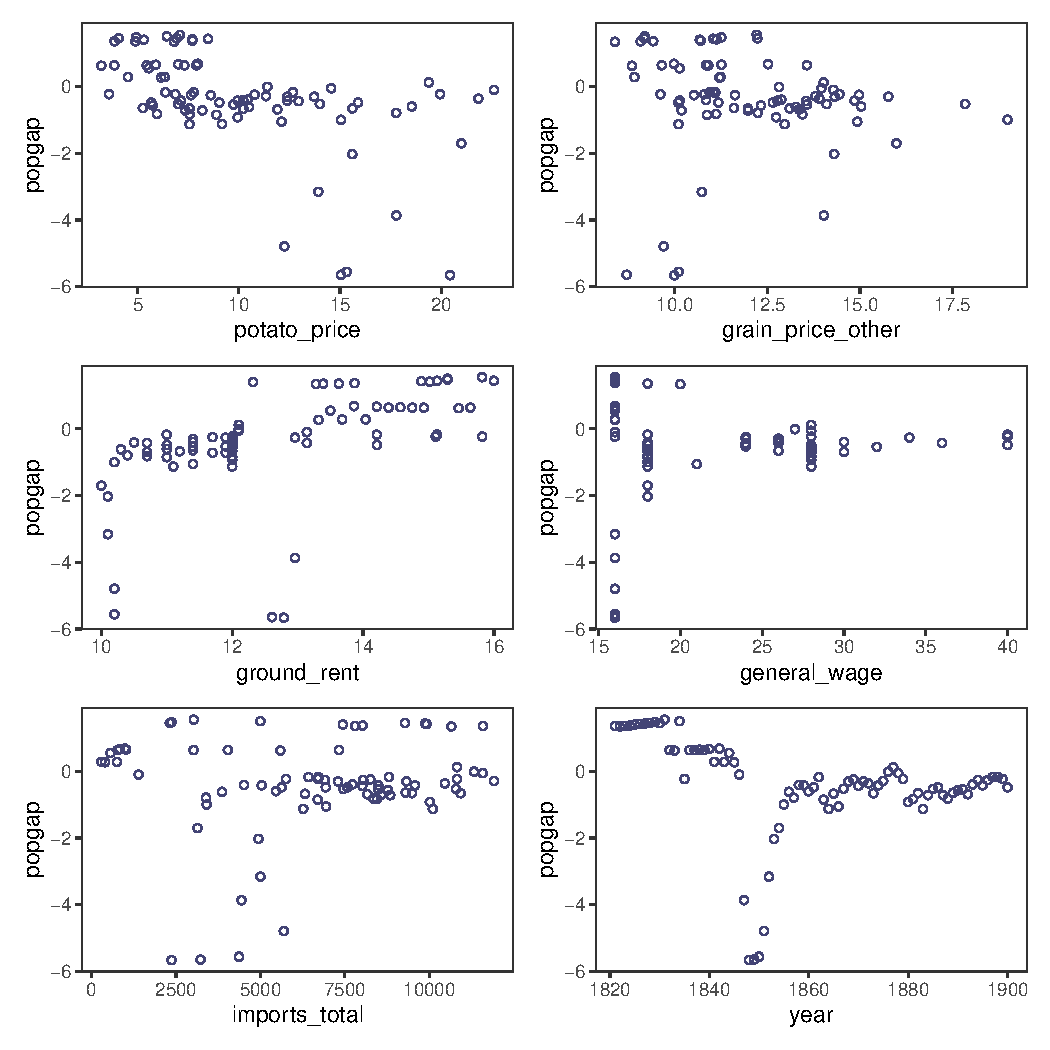
\includegraphics[width=.95\textwidth]{../03_outputs/regression_scatter.pdf}
\end{figure}

Therefore, generalized additive model was used as the main approach in this paper since it is efficient in solving non-linearly relationship from variables by using smooth functions. Wood demonstrates the usability of the GAM method in non-linear data and reduces the risk of over-fitting by introducing penalty coefficients in corresponding calculations \citep{wood2001mgcv}. Recent studies in the demographic have shown the GAM approach possesses a more significant performance than the GLM approach in fitting regressions \citep{potts2018evaluation}. In addition, there are scholars who used GAM for entitlement analysis \citep{ardyanto2006granting}, and also performed a good fit between GAM and entitlement research.

Variables in regression included: \texttt{potato\_price}, \texttt{grain\_price\_other}, \texttt{ground\_rent}, \texttt{if\_tithe}, \texttt{general\_wage}, \texttt{poorlaw}, \texttt{imports\_total}, \texttt{exports\_total}. The second regression model includes the variables \texttt{grain\_acre\_total}. Based on the observation of scatter and correlation matrix, a smoothing function was added to the variables \texttt{grain\_price\_other}, \texttt{general\_wage}, and \texttt{exports\_total}. 

Imports and exports data was used as control variable due to literatures that can be examined. This data during famines have always been a focus of debate among different schools, because differences in views will directly lead to the division between nationalism and revisionism \textemdash\ to put it more bluntly, it determines whether scholars will target 19th century's British government. 

\begin{itemize}
    \item [] \textit{``During all the famine year, Ireland actually producing sufficient food, and wool and flax to feed and clothe not nine, but eighteen millions of people''.} \citep{mitchel1905apology}
    \item [] \textit{``At least, historians of Ireland, even the native-born ones, taking them as a group, were not as revisionist in their perspective''.}\citep{donnelly1996construction}
\end{itemize}

The first advantage of using this part of data as a control variable is that it maintains what Weber called value neutrality. Not using import/export data to validate the hypothesis is essentially stepping outside the discourse of the nationalism/revisionism debate and using the precondition of ``in the presence of consistent import/export data'' to examine changes in the entitlements. Secondly, the imports and exports amount will directly related to the domestic economic, as scholars \citep{hansard1840flour} pointed out in 19th century with a research in the transactions between Ireland and UK, in turn, create a chain reaction on everyday life in terms of price indices, market coverage, etc, as well as having an impact on the population and cultivation of the country \citep{solar2015ireland}. To summarize, both from a neutral point in view of the theoretical and from a precise point in the view of analysis, imports and exports data should be controlled when discussing people's entitlements.

The formulation of the regression model is written below, including the assumptions represented by each variable, smooth term and control variables:

\vspace{-14pt}
\begin{align*}
\texttt{E(popgap)} = & \ \beta_0 + \beta_1 \times \texttt{potato\_price} + f_1(\texttt{grain\_price\_other}) \ldots \textit{(H1)} \\
                & + \beta_2 \times \texttt{ground\_rent} + \beta_3 \times \texttt{factor(if\_tithe)} \ldots \ldots .. \textit{(H2)} \\
                & + f_2(\texttt{general\_wage}) \ldots \ldots \ldots \ldots \ldots \ldots \ldots \ldots \ldots \ldots \ldots . \textit{(H3)} \\
                & + \beta_4 \times \texttt{factor(poorlaw)} \ldots \ldots \ldots \ldots \ldots \ldots \ldots \ldots \ldots . .. \textit{(H4)} \\
                & + \beta_5 \times \texttt{imports\_total} + f_3(\texttt{exports\_total}) \ldots Controlled\\
                & + \epsilon
\end{align*}
\vspace{-2cm}
\begin{align*}
\texttt{popgap} = & \ \beta_0 + \beta_1 \times \texttt{grain\_acre\_total}  \ldots \ldots \ldots  \ldots \ldots \ldots \ldots \ldots (\textit{H5a/5b}) \\
& + \beta_5 \times \texttt{imports\_total} + + \beta_6 \times \texttt{exports\_total} \ldots Controlled\\
& + \epsilon
\end{align*}

\section{Assumptions Test}

This paper fits two regression model. The first regression model is a GAM model, which is used to prove \textit{H1}, \textit{H2}, \textit{H3} and \textit{H4}; the second regression model, due to the linear relationship between variables \texttt{grain\_acre\_total} and \texttt{popgap}, is a linear regression, which is used to prove \textit{H5}. In fact, for the second regression model, the linear regression and the GAM model have the same AIC, and to follow the modeling principle of simplicity, linear regression is used for fitting.

The necessity and feasibility for the use of the GAM must be justified before proceeding with the regression analysis. The first is the test of multicollinearity. Although GAM is not as sensitive to multicollinearity as linear regression due to the introduction of the smoothing function, however, excessive correlation between independent variables can still lead to errors in stability and explanations ability in the regression results, so the corresponding VIF test is necessary. The results of VIF test shows in Table 4.1, which indicates independence among the variables of the regression model is satisfied and there are no highly correlated independent variables.

\begin{table}[h] \centering 
    \caption{Model Variance Inflation Factors (VIF)} 
    \label{vif_table} 
    \begin{tabular}{lcccc} 
    \\[-1.8ex]\hline 
    \hline \\[-1.8ex] 
    Variable & VIF & Variable & VIF \\ 
    \hline \\[-1.8ex] 
    potato\_price & 2.044 & general\_wage & 5.390 \\ 
    grain\_price\_other & 1.739 & imports\_total & 6.844 \\ 
    ground\_rent & 3.716 & exports\_total & 1.918 \\ 
    factor(if\_tithe)1 & 5.666 & factor(poorlaw)1 & 4.606 \\ 
    \hline 
    \hline \\[-1.8ex] 
    \end{tabular} 
\end{table}

The model was tested with \texttt{gam.check()} in \texttt{R}, returning results in Figure 4.2.

\begin{figure}[h]
    \centering
    \caption{Regression Check}
    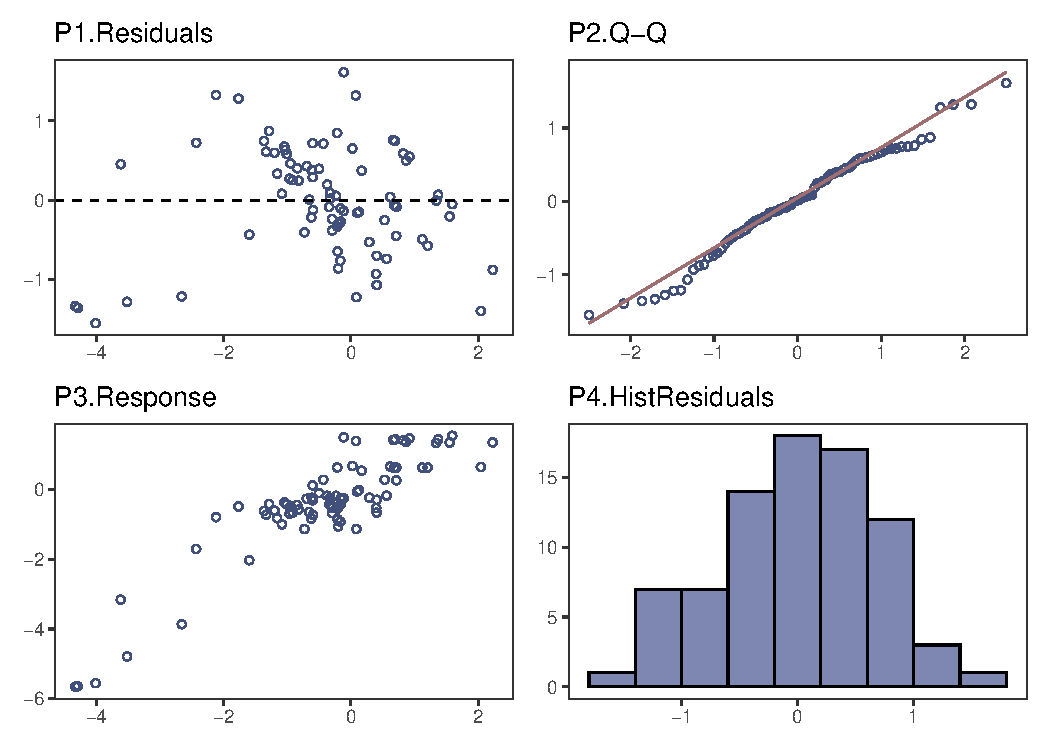
\includegraphics[width=.9\textwidth]{../03_outputs/regcheck.pdf}
\end{figure}
\vspace{-7pt}

From $P1$, it appears that the distribution of the residuals revolves around the $Y=0$ line with a mean approximately equal to 0 and no pattern can be found; whereas the Q-Q plot of $P2$ indicates a normal distribution structure of the data; $P3$ also shows a uniform and random distribution between the response value and fitting value; and finally, the residuals indicated by $P4$ show a normal distribution.

It is also important to state the advantages of using GAM over using LM for the data format of this study. GAM was found to have a significantly higher R-squared and a lower AIC compared with LM. Figure 4.2 shows the details:

\begin{table}[h] 
    \centering 
    \caption{Regression Results: GAM and Linear} 
  \begin{tabular}{@{\extracolsep{5pt}}lcc} 
  \\[-1.8ex]\hline 
  \hline \\[-1.8ex] 
   & \multicolumn{2}{c}{\textit{Dependent variable:}} \\ 
  \cline{2-3} 
  \\[-1.8ex] & \multicolumn{2}{c}{popgap} \\ 
  \hline \\[-1.8ex] 
   & GAM & LM \\ 
  \hline \\[-1.8ex] 
  \multicolumn{3}{c}{Coefficients are omitted to save space and will be shown in next Chapter} \\
  \hline \\[-1.8ex] 
  Observations & 80 & 80 \\ 
  Adjusted R$^{2}$ & 0.741 & 0.570 \\ 
  AIC & 201.470 & 235.916\\
  Residual Std. Error &  & 0.990 (df = 71) \\ 
  F Statistic &  & 14.115$^{***}$ (df = 8; 71) \\ 
  \hline 
  \hline \\[-1.8ex] 
  \textit{Note:}  & \multicolumn{2}{r}{$^{*}$p$<$0.1; $^{**}$p$<$0.05; $^{***}$p$<$0.01} \\ 
  \end{tabular} 
\end{table} 

\section{Regression Results}

Based on regression results (Table 4.3, row GAM), we can interpret the coefficients: in terms of the trade-based entitlement, an 1 unit increase in the price of potatoes, the population change within a year is associated with an average increase of -7\%; In terms of the production-based entitlement, an 1 unit increase in the ground rent, the population change within a year is associated with an average increase of 34\%, but maybe due to \texttt{if\_tithe} use a binary form to describe the effect between tithe and population change and the year of compulsory tithe is not many during century, so the coefficient is not significant ($p=0.424$); In terms of the own-labour entitlement, there is a significant relationship between wage and population change can be observed, and it will be more clear explained in the smooth term interpret part; In terms of the inheritance and transfer entitlement, years with Poor Law will have an average 36\% increase in population change compared with years without Poor Law. 

A description of the control variables reveals that an 1 unit increase in the imports amount, the population change within a year is associated with an average increase of 4\%, which is fit to the empirical knowledge and as well as part of the transfer and inheritance entitlement. But there is no significant relationship be observed between the exports grain amount and population change,

Further data-based rebuttals to the FAD theory can be made here. The only significant coefficient under 10\% confidence level in the model is grain import amount ($p=0.055$), and regarding grain planting acreage and export amount, they are all non-significant, i.e., there is no relationship between planting acreage and population change, as well as export food amount, which prove \textit{H5}: \textbf{There is not enough evidence to suggest that larger planting acreage lead to an increase in population compared with last year}. 

\begin{table}[h]
    \centering
    \caption{GAM, FAD LM, and General LM}
    \begin{tabular}{@{\extracolsep{5pt}}lccc}
    \\[-1.8ex]\hline
    \hline \\[-1.8ex]
    & \multicolumn{3}{c}{\textit{Dependent variable: popgap}} \\
    \cline{2-4}
    \\[-1.8ex] & GAM & FAD LM & General LM \\
    \hline \\[-1.8ex]
    potato\_price & $-$0.079$^{***}$ & & $-$0.107$^{***}$ \\
     & (0.028) & & (0.033) \\
    grain\_price\_other & &  & 0.179$^{**}$ \\
     & &  & (0.069) \\
    grain\_acre\_total & & $-$0.002 & \\
     & & (0.001) & \\
    ground\_rent & 0.342$^{***}$ & & 0.082 \\
     & (0.118) & & (0.119) \\
    factor(if\_tithe)1 & 0.450 & & 1.159$^{**}$ \\
     & (0.559) & & (0.535) \\
    general\_wage & & & 0.050 \\
     & & & (0.037) \\
    factor(poorlaw)1 & 3.616$^{***}$ & & 3.103$^{***}$ \\
     & (0.617) & & (0.752) \\
    imports\_total & 0.044$^{***}$ & 0.014$^{*}$ & 0.042$^{***}$ \\
     & (0.008) & (0.007) & (0.010) \\
    exports\_total & & 0.0003 & 0.001 \\
     & & (0.001) & (0.001) \\

    Constant & $-$7.420$^{***}$ & $-$0.072 & $-$7.751$^{***}$ \\
     & (1.391) & (1.686) & (1.964) \\
    \hline \\[-1.8ex]
    s(grain\_price\_other) & $^{**}$ & & \\
    s(general\_wage) & $^{***}$ & & \\
    s(exports\_total) &  & & \\
    \hline \\[-1.8ex]
    Observations & 80 & 80 & 80 \\
    Adjusted R$^{2}$ & 0.741 & 0.127 & 0.570 \\
    AIC & 201.470 & & 235.916 \\
    Residual Std. Error & & 1.412 (df = 76) & 0.990 (df = 71) \\
    F Statistic & & 4.827$^{***}$ (df = 3; 76) & 14.115$^{***}$ (df = 8; 71) \\
    \hline
    \hline \\[-1.8ex]
    \textit{Note:}  & \multicolumn{3}{r}{$^{*}$p$<$0.1; $^{**}$p$<$0.05; $^{***}$p$<$0.01} \\
    \end{tabular}
\end{table}

Figure 4.3 visualizes the smooth term and describes the relationship between smooth term and population change. The smooth term \texttt{exports\_total}, due to it is imported to model as control variable firstly, and not significance secondly, is not showed:

\begin{figure}[h]
    \centering
    \caption{Significant Smooth Term Plot}
    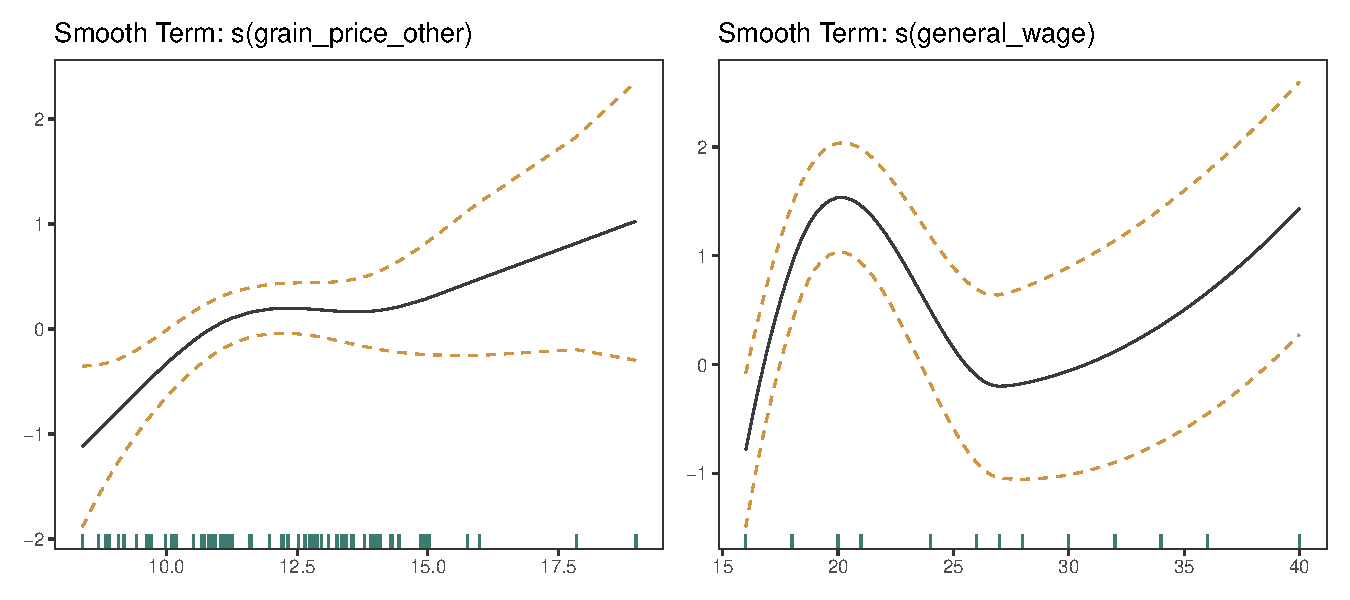
\includegraphics[width=.95\textwidth]{../03_outputs/smoothterm.pdf}
\end{figure}

Regarding the relationship between other grain price and population, we can see a positive relationship from approximately 8.5 to 12, then stable till 15, and then positive again. A possible explanation would be when grain price grows in lower price interval, it related to the profit of peasant, which makes a increase in population, while when it grows in high price interval, it related to a price index increase due to the development of the whole society. As for middle price interval, with price rise there is a no or even negative correlation between dependent and independent variables.

Regarding the relationship between wage and population, we can see a positive relationship from 16 to 21, then negative relationship from 21 to 26, finally appears to positive again. This paper argues this trend change is also due to the fact that the people benefit at the beginning when wages increase, and that the increase in the middle range of wages is perhaps linked to inflation, while the increase in the high range is the general development of the society. 

A more details logic related to this smooth term trend will be discussed in the Chapter 5.1, which will be presented associated with the interpret of results. 

\newpage

\section{Robustness Test}

The GAM of this paper is tested for robustness, and the main methods include replacing the model, adding independent variables, changing the sample range, and changing the treatment of missing values. The results are presented in Table 4.4.

Firstly, as mentioned earlier, the robustness of GAM is tested using a linear regression model (Model 2). Compared to GAM, the LM shows differences in the coefficient assignments of $H2$, mainly the insignificant coefficient of land rent and the significant coefficient of tithe. This difference is acceptable because both are used to describe production-based entitlement, and therefore small differences in the coefficients in the same hypothesis are not sufficient to indicate that the model is not robust. Otherwise, all other coefficients of LM are generally consistent with the GAM.

Secondly, variable \texttt{year} is put into the model (Model 3) to exclude the influence between year and population, e.g., industrial revolution, land war, etc. The coefficients are stable after adding variable \texttt{year}.

Thirdly, due to the mechanism of population change maybe different during time, which is suggested by typical Modernization theory \citep{tipps1973modernization} in development field, and Ireland may be considered as a pre-modern society before famine and development rapidly at the end of 19th century, so it is necessary to cut half observations to clear the influence if it exist (Model 4). The results also shows a similar coefficient, except the coefficient of potato price appears a stronger negative trend than standard GAM due to the effect of famine is enlarged in the first half of 19th century.

Lastly, as mentioned before, this paper use multiple imputation to deal with missing value in ground rent, import and export data, and to valid the robustness of GAM, regression imputation will be conducted to create a new model to compare. Also, similar coefficients are appeared after changing imputation method. 

In a word, the robustness of the GAM receives support from multiple models, which means the conclusion of GAM has a good credibility.

\begin{table}[h]
    \centering
    \caption{Robustness Test}
    \begin{tabular}{@{\extracolsep{5pt}}lccccc}
    \\[-1.8ex]\hline
    \hline \\[-1.8ex]
    & \multicolumn{5}{c}{\textit{Dependent variable: popgap}} \\
    \cline{2-6}
    \\[-1.8ex] & Model 1 & Model 2 & Model 3 & Model 4 & Model 5 \\
    & \textit{standard} & \textit{linear} & \textit{year} & \textit{half} & \textit{mice} \\
    \hline \\[-1.8ex]
    potato\_price & $-$0.079$^{***}$ & $-$0.107$^{***}$ & $-$0.096$^{**}$ & $-$0.133$^{**}$ & $-$0.063$^{*}$ \\
     & (0.028) & (0.033) & (0.028) & (0.050) & (0.025) \\
    grain\_price\_other & & 0.178$^{*}$ &  & & \\
     & & (0.069) &  & & \\
    ground\_rent & 0.342$^{***}$ & 0.082 & 0.306$^{*}$ & 0.266$^{.}$ & 0.323$^{**}$ \\
     & (0.118) & (0.119) & (0.123) & (0.155) & (0.111) \\
    factor(if\_tithe)1 & 0.450 & 1.159$^{*}$ & 0.905 & 1.999$^{.}$ & 0.924$^{.}$ \\
     & (0.559) & (0.535) & (0.610) & (1.086) & (0.509) \\
    general\_wage & & 0.050 & & 1.021$^{***}$ & 1.021$^{***}$ \\
     & & (0.037) & & (0.261) & (0.261) \\
    factor(poorlaw)1 & 3.616$^{***}$ & 3.103$^{***}$ & 2.867$^{***}$ & 3.832$^{***}$ & 3.812$^{***}$ \\
     & (0.617) & (0.752) & (0.664) & (0.901) & (0.523) \\
    imports\_total & 0.044$^{***}$ & 0.042$^{***}$ & 0.032$^{***}$ & 0.049$^{***}$ & 0.056$^{***}$ \\
     & (0.008) & (0.010) & (0.009) & (0.012) & (0.008) \\
    exports\_total & & 0.001 & & & \\
     & & (0.001) & & & \\
    year & & & -0.004$^{*}$ & & \\
     & & & (0.017) & & \\ 

    \hline \\[-1.8ex]
    s(grain\_price\_other) & $^{**}$ & & $^{**}$ & $^{*}$ & $^{***}$  \\
    s(general\_wage) & $^{***}$ & & $^{***}$ & & $^{***}$ \\
    s(exports\_total) & & & \\
    \hline \\[-1.8ex]
    Observations & 80 & 80 & 80 & 40 & 80 \\
    \hline
    \hline \\[-1.8ex]
    \textit{Note:} & \multicolumn{5}{r}{$^{*}$p$<$0.1; $^{**}$p$<$0.05; $^{***}$p$<$0.01} \\
    \end{tabular}
\end{table}

During the creating of different models, the influence of potato price, as well as the smooth term, is significant in every models, which gives a strong evidence of the relationship between the trade-based entitlement and population change. The secondly common significance appears in the Poor Law, and this also makes a comprehensive conclusion that Poor Law increase peoples' entitlement in transfer and inheritance. General wage shows the similar situation and can be found significance in either regular term or smooth term either. As for ground rent, after adding variable \texttt{year}, in Model 3 and Model 4 it is losing significance, which is caused by the history events caused by history like land war or related laws.

\newpage

\section{Research Design}

Before further discuss the findings, it is necessary to review the research logic.

Firstly is the theoretical framework: (1) entitlement approach used by Amartya Sen in his book ``Poverty and Famine'', and (2) refutation of the FAD theory. According to Sen's construct, the entitlement approach consists of the following four indicators: trade-based entitlement, production-based entitlement, own-labour entitlement and Inheritance and transfer entitlement; while the FAD theory includes one indicator, the area under food cultivation. This paper generalizes the entitlement approach as a demographic and developmental mechanism based on the literature and attempts to explore if the changes in people's entitlements, which is the independent variable, will affect population change within the year, which is the dependent variable.

Further, hypotheses are made base on these indicators, with each indicator corresponding to a hypothesis and each hypothesis corresponding to more specific variables in the dataset. $H1$ corresponds to price of grains, $H2$ corresponds to ground rent and presence or absence of tithing, $H3$ corresponds to general wage, $H4$ corresponds to the Poor Law, and $H5$ corresponds to the grain planting acreage. Import and Export amount were used as control variables into regression model.

The GAM was used in this study for a number of reasons, including (1) there is no significant linear relationship between some independent variables and the dependent variable, but there is an observable nonlinear relationship and theory supports the existence of such a nonlinear relationship, and (2) the introduction of a smoothing function in the GAM can predict this nonlinear relationship in a good way. Relative examines have been performed before formally discussing the regression, including the VIF test for multicollinearity, AIC and R-square comparisons for linear regression, the residual randomness and normality test, and robustness test. All of the results identify the GAM as a reasonable regression model under this data.

Figure 4.4 visualizes the framework of the entire research.

\begin{landscape}
    \begin{figure}[h]
        \centering
        \caption{Research Design}
        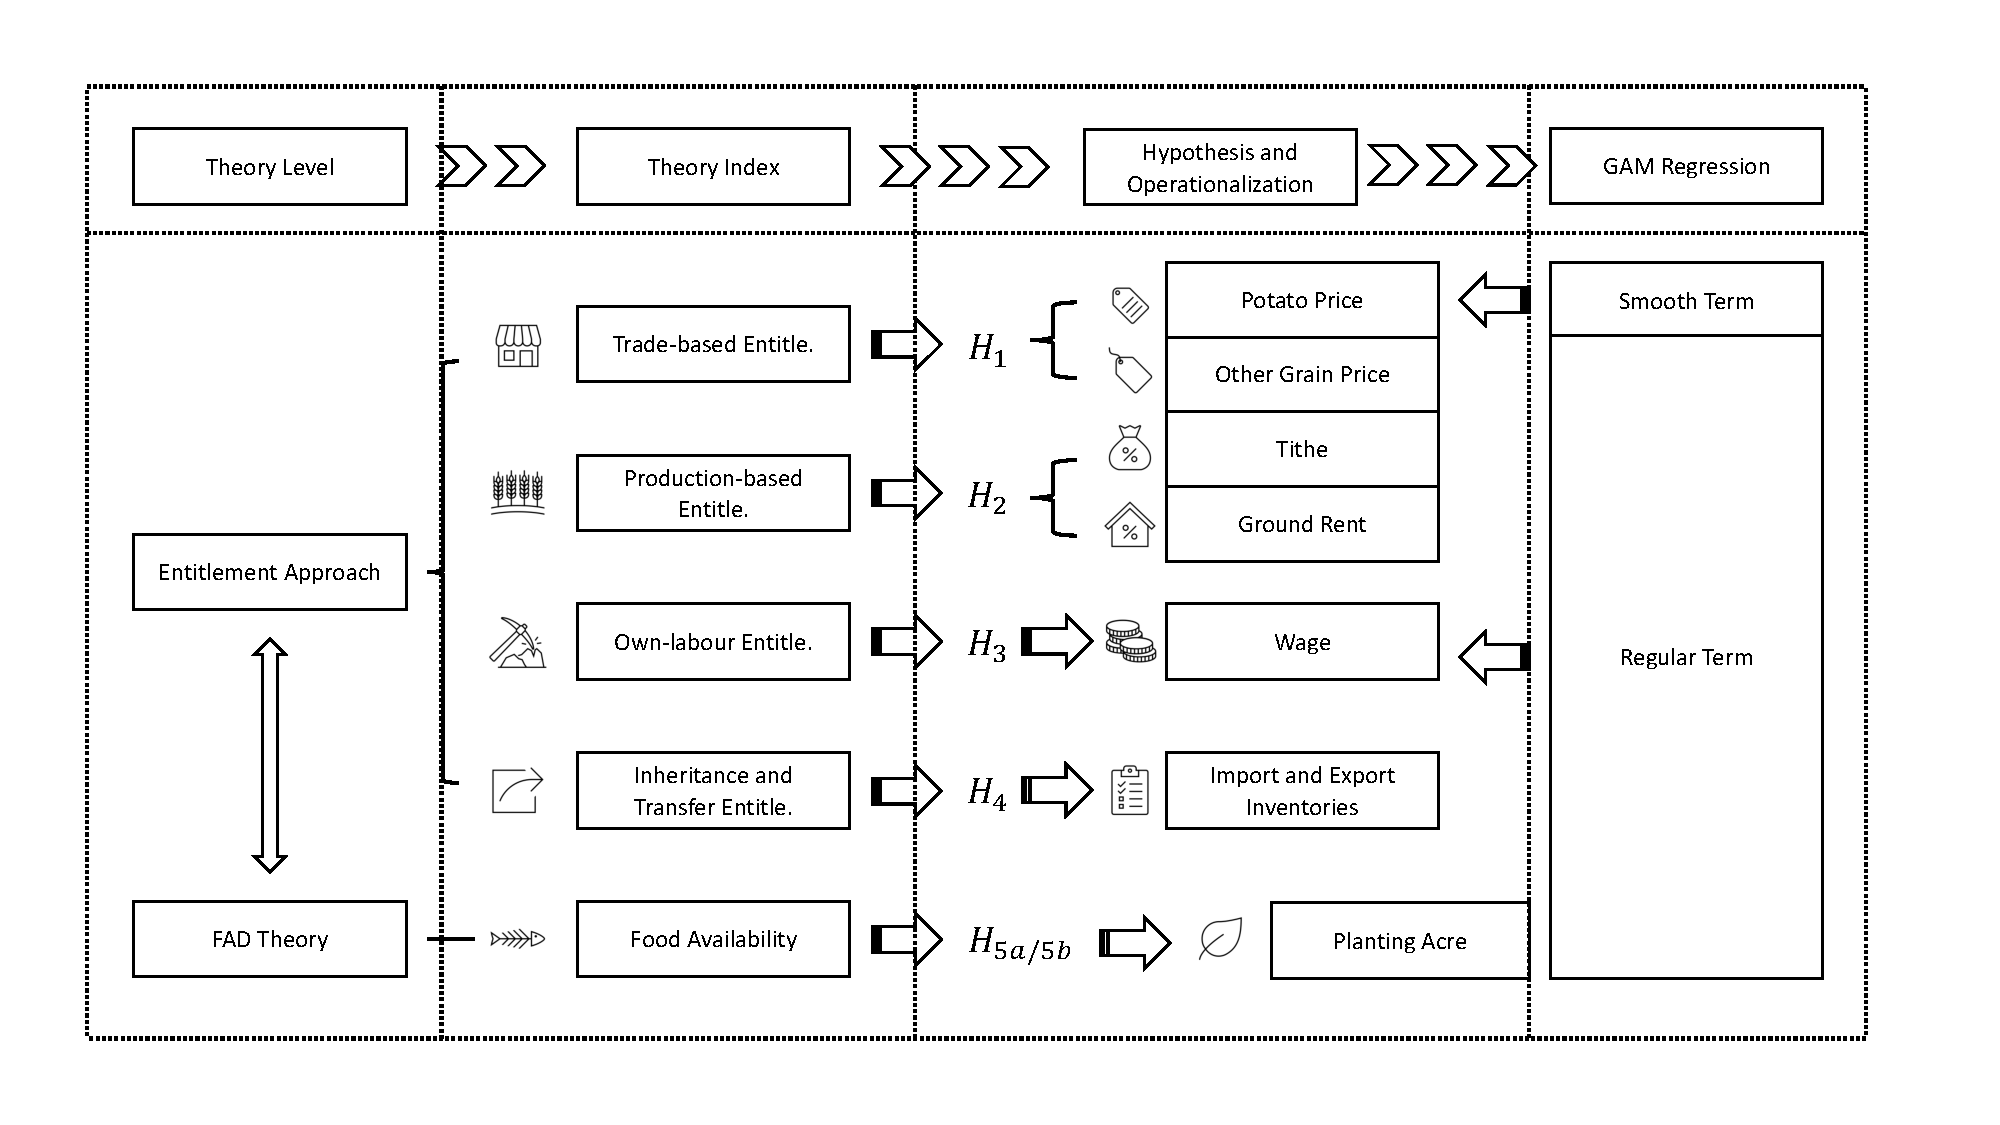
\includegraphics[width=1.5\textheight]{../03_outputs/Framework.pdf}
    \end{figure}
\end{landscape}
